\section{\textsc{Noise Functions}}
\hrule height 0.5pt
\vspace*{2.5pt}

\subsection{\textsc{Theory}}
\vspace*{-10pt}

Let $\EuScript{N}:\R^n\rightarrow\R$ denote the core noise function, where $n$ is the dimensionality of the
input domain. As mentioned in the introduction, there exist two variants: 
Value noise, $\EuScript{N}_V$, and Perlin noise, $\EuScript{N}_P$.

This IA specifically focuses on the two-dimensional case, where the noise generation algorithm operates on
a pixel grid of resolution $N\times N$ iterating over integer coordinates $(u,v)\in\{0,1,\dots,N-1\}^2$. As
established in the introduction, $N=256$. These discrete coordinates are transformed into the normalised domain 
$Q_\text{base}=[0,1)^2\subset\Q^2$ via the transformation $(x,y)=\left(\dfrac{u}{N},\dfrac{v}{N}\right)$. This 
ensures scale invariance, guaranteeing that relative feature positions remain constant under resolution change. 

Let $G_V:\Z^2\rightarrow[0,1]$ and $\vec{G}_P:\Z^2\rightarrow \R^2$ be lattice functions associated with Value noise and 
Perlin noise, respectively. For a domain $0\le i,j\le N$, these functions map integer lattice coordinates to precomputed
random values as follows:
\begin{itemize}
    \item $G_V(i,j)$ returns a pseudorandom scalar $v_{i,j}\in[0,1]$, sampled uniformly.
    \item $\vec{G}_P(i,j)$ returns a pseudorandom unit vector $\hat{v}_{i,j}$ sampled uniformly. 
\end{itemize}
For any query point $(x,y)\in Q_\text{base}$, and let $(i,j)$ be the coordinate of the top-left vertex associated with the
chosen query coordinate, then because all vertex coordinates are integer pairs, the value of $i$ and $j$ can be found by rounding
$x$ and $y$ down to the nearest integer, which is written as the floor function.
\[i=\lfloor x\rfloor,j=\lfloor y\rfloor\] 
Subsequently, the associated top-right, bottom-right, and bottom-left vertices are respectively $(i+1,j)$, $(i+1,j+1)$, and $(i,j+1)$.

Finally, interpolate the query point with the values at the four lattice vertices to obtain the height value at the query point. Although
bicubic and spline interpolations are possible, due to the limited scope of this IA, we will only be exploring bilinear interpolation with 
different polynomial smoothstep function $S_n(t)$, where $n$ is the order of the function. 

To derive the formula for bilinear interpolation, we first interpolate in the $x$-direction which yields two intermediate values
\begin{align*}
    \begin{cases}
        \EuScript{N}(x,j)=\EuScript{N}(i,j)\cdot(1-S_n(x-i))+\EuScript{N}(i+1,j)\cdot S_n(x-i)\\
        \EuScript{N}(x,j+1)=\EuScript{N}(i,j+1)\cdot(1-S_n(x-i))+\EuScript{N}(i+1,j+1)\cdot S_n(x-i)
    \end{cases}
\end{align*}
Substitute $\EuScript{N}(i,j)$, $\EuScript{N}(i+1,j)$, $\EuScript{N}(i,j+1)$, and $\EuScript{N}(i+1,j+1)$ with $G_V(i,j)$, $G_V(i+1,j)$,
$G_V(i,j+1)$, and $G_V(i+1,j+1)$ respectively
\begin{align*}
    \begin{cases}
        \EuScript{N}(x,j)=G_V(i,j)\cdot(1-S_n(x-i))+G_V(i+1,j)\cdot S_n(x-i)\\
        \EuScript{N}(x,j+1)=G_V(i,j+1)\cdot(1-S_n(x-i))+G_V(i+1,j+1)\cdot S_n(x-i)
    \end{cases}
\end{align*}
We then interpolate in the $y$-direction, yielding our height value
\begin{align*}
    \EuScript{N}_V(x,y)=&\EuScript{N}_V(x,j)\cdot(1-S_n(y-j))+\EuScript{N}_V(x,j+1)\cdot S_n(y-j) \\
    =&[G_V(i,j)\cdot(1-S_n(x-i))+G_V(i+1,j)\cdot S_n(x-i)]\cdot(1-S_n(y-j))\\
    &+[G_V(i,j+1)\cdot(1-S_n(x-i))+G_V(i+1,j+1)\cdot S_n(x-i)]\cdot S_n(y-j)
\end{align*}
which can be condensed into the matrix expression
\begin{equation} \label{eq:1}
    \EuScript{N}_V(x,y)=
    \begin{bmatrix}
        1-S_n(x-i) & S_n(x-i)
    \end{bmatrix}
    \begin{bmatrix}
        G_V(i,j) & G_V(i+1,j)\\
        G_V(i,j+1) & G_V(i+1,j+1)
    \end{bmatrix}
    \begin{bmatrix}
        1-S_n(y-j)\\
        S_n(y-j)
    \end{bmatrix}
\end{equation}
Equation \ref{eq:1} can be modified to suit $\EuScript{N}_P(x,y)$ by replacing $G_V(i,j)$ with the
dot product $g_{i,j}=\vec{G}_P(i,j)\cdot \vec{r}_{i,j}$, where $\vec{r}_{i,j}$ is the displacement vector from
point $(x,y)$ to $(i,j)$.

To generate a full terrain, repeat the above steps for all query points $(x,y)$. 

\subsection{\textsc{Key Parameters}}
\vspace*{-10pt}

To control the characteristics of a noise function, we can introduce two adjustable parameters: frequency and 
amplitude. Frequency, $0<\lambda\le\frac{N}{2}$, determines the density of features within the terrain - greater 
frequency leads to more granular details. The upper bound on frequency derives from the Nyquist-Shannon sampling 
theorem, which, according to Candes and Wakin (2008), states that “the sampling rate must be at least twice the 
maximum frequency present in the signal.” Consequently, having integrated frequency into account, the effective 
domain of the noise function now becomes $Q=[0,\lambda)^2$. Amplitude, $A>0$, defines the overall magnitude of the
noise function - where $A>1$ lead to greater extremes in the terrain elevation while $0<A<1$ leads to less extremes.

Incorporating both parameters, we modify the noise function as follows
\[A\cdot\EuScript{N}(\lambda x,\lambda y)\]
Next, recall that the smoothstep function $S_n(t)$ serves as an interpolation weight in noise functions, as seen in 
Equation \ref{eq:1}. It must satisfy the following conditions:
\begin{itemize}
    \item \textbf{Boundary conditions:} $S_n(0)=0$ and $S_n(1)=1$.
    \item \textbf{Continuity:} for $m=1,2,\dots,\lfloor\frac{n}{2}\rfloor$, the $m^{\text{th}}$ derivative of $S_n$ satisfies 
    $S_n^{(m)}(0)=0$ and $S_n^{(m)}(1)=0$. The floor function ensures $m$ is an integer, as fractional derivatives are
    not considered here.
    \item \textbf{Monotonicity} (strictly increasing): $S_n'(t)>0,\forall t\in(0,1)$
    \item \textbf{Rotational symmetry about $(0.5,0.5)$:} This condition can be derived by first defining a shifted function that centers
    the point of symmetry at the origin:
    \[f(u)=S_n\left(u+\frac{1}{2}\right)-\frac{1}{2}\]
    then enforcing conditions of an odd function to enforce symmetry:
    \begin{align*}
        f(-u)&=-f(u)\\
        S_n\left(-u+\frac{1}{2}\right)-\frac{1}{2}&=-\left[S_n\left(u+\frac{1}{2}\right)-\frac{1}{2}\right]
    \end{align*}
    Finally, substituting $t=\frac{1}{2}-u$, then simplify:
    \begin{align*}
        S_n(t)-\frac{1}{2}&=-\left[S_n(1-t)-\frac{1}{2}\right]\\
        S_n(t)&=1-S_n(1-t)
    \end{align*}
\end{itemize}
Having established the conditions, we will now attempt to construct a smoothstep function by first giving it the general form of
a polynomial
\[S_n(t)=\sum_{k=0}^{n}a_kt^k\]
where $a_k$ is the coefficient of the $k^{\text{th}}$ term.

From the symmetry condition, it follows that $n$ must be odd (Wikimedia Foundation, 2025). Although I attempted to formally prove 
this result, I was unable to reach a conclusive one. Therefore, for the purposes of this Internal Assessment, this property will 
be assumed to hold.

From the continuity condition $S_n^{(m)}(1)=0$, we know that there is no constant term in any of the derivative up to 
$m=\lfloor\frac{n}{2}\rfloor$, hence the lowest-order term in the polynomial $S_n(t)$ is $t^{\lfloor\frac{n}{2}\rfloor+1}$. This is
because each term in the polynomial contributes a non-zero constant to the $m^{\text{th}}$ derivative at $t=1$ when $k\le m$. By
eliminating all terms where $k\le \lfloor\frac{1}{2}\rfloor$, we ensure that every required derivative automatically vanishes at 
the endpoint. Amending this finding, we rewrite the smoothstep function as
\[S_n(t)=\sum_{k=\lfloor\frac{n}{2}\rfloor+1}^{n}a_kt^k\]
We now see another benefit of the floor function for $\frac{n}{2}$, which is to ensure that the index $k$ in the sigma summation is 
always an integer. We might have also noticed that there is no upper-bound for $n$, which means that infinitely many smoothstep functions 
are available. For this investigation, I limit consideration to cubic and quintic polynomials, as higher-degree polynomials will introduce 
too many coefficients to solve for, as well as costing computation time. 

With all the conditions and boundaries set, we aim to analytically solve for $S_3(t)$ defined as:
\[S_3(t)=a_2t^2+a_3t^3\]
Applying the boundary condition and continuity condition, we obtain the simultaneous equation:
\begin{align}
    \begin{cases*}
        \sum_{k=2}^{3}a_k=1\\
        S_3'(1)=0
    \end{cases*}
    \implies
    \begin{cases*}
        a_2+a_3=1\quad\quad \text{\textcircled{\footnotesize{A}}} \\
        2a_2+3a_3=0\quad \text{\textcircled{\footnotesize{B}}}
    \end{cases*}
\end{align}

Rewrite equation 2A in terms of $a_3$
\[a_3=1-a_2\]
then substitute into equation 2B
\begin{align*}
    2a_2+3(1-a_2)&=0\\
    2a_2+3-3a_2&=0\\
    a_2&=3
\end{align*}
Now, substitute the value of $a_2$ back into equation 2A
\[a_3=1-(3)=-2\]
Thus, the smoothstep function of order 3 becomes:
\begin{equation} \label{eq:3}
    S_3 (t)=-2t^3+3t^2
\end{equation}
As mentioned, we will also attempt to derive the quintic smoothstep function $S_5(t)$
\[S_5(t)=a_3t^3+a_4t^4+a_5t^5\]
Applying the continuity and boundary condition:
\begin{align}
    \begin{cases*}
        \sum_{k=3}^{5}a_k=1 \\
        S_5'(1)=0 \\
        S_5''(1)=0
    \end{cases*}
    \implies
    \begin{cases*}
        a_3+a_4+a_5=1\\
        3a_3+4a_4+5a_5=0\\
        6a_3+12a_4+20a_5=0
    \end{cases*}
    \implies
    \begin{cases*}
        a_3+a_4+a_5=1\\
        3a_3+4a_4+5a_5=0\\
        3a_3+6a_4+10a_5=0
    \end{cases*}
\end{align}

PUT GAUSSIAN ELIMINATION STUFF HERE LATER

There are two other parameters we will adress: persistence and lacunarity. Typically, a noise function with a single frequency will look 
overly smooth and artificial. Natural terrains, on the other hand, exhibit complexity at multiple scales. For instance, a mountain presents broad overall forms alongside finer features such 
as ridges and crevices layered atop one another.

To replicate the complexity of natural terrains, fractal noise is used where multiple layers of noise (called octaves) are summed, each with 
decreasing amplitude and increasing frequency. The parameter persistence, $0<P<1$, controls the rate at which amplitude decay, ensuring higher 
frequency details do not overwhelm the overall coherence. Lacunarity, $L>1$, determines the rate of frequency growth, introducing finer-scale 
variations. Commonly, the value of $P$ and $L$ is chosen such that $P\cdot L=1$. Finally, the total number of octaves, $C\ge 1$, controls the level of detail in the terrain. Putting this together, the final terrain 
height at pixel $(u,v)$ is given by:
\[\EuScript{N}_{FV}(x,y)=\sum_{k=0}^{C-1}A_k\cdot\EuScript{N}_V\left(\lambda_k\frac{u}{N},\lambda_k\frac{v}{N}\right)\]
where
\begin{itemize}
    \item $A_k=A_0\cdot P^k$
    \item $\lambda_k=\lambda_0\cdot L^k$
\end{itemize}
$\EuScript{N}_V$ can be replaced by $\EuScript{N}_P$, and thus $\EuScript{N}_{FV}(x,y)$ to $\EuScript{N}_{FP}(x,y)$, depending on which noise variant 
is being used. One final detail is determining the upper bound for $C$. Recall that $\lambda_{C-1}$ must satisfy the Nyquist limit mentioned earlier, 
which gives us the inequality:
\begin{align*}
    \lambda_{C-1}&\le \frac{N}{2}\\
    \lambda_0\cdot L^{C-1} &\le \frac{N}{2}\\
    L^{C-1} &\le \frac{N}{2\lambda_0}\\
    C &\le 1+\log_L\left(\frac{N}{2\lambda_0}\right)
\end{align*}
Having introduced the core theory and parameters in this IA, I will now present the quantitative tools that will be used to compare the noise functions.

\subsection{\textsc{Quantitative Metrics}} \label{quant_metrics}
\vspace*{-10pt}

Firstly, all elevation values generated from noise functions are aggregated and plotted onto a histogram to analyze their statistical distribution. The 
number of intervals were determined using Rice rule, a preferred method which “set the number of intervals to twice the cube root of the number of 
observations.” (Lane \& Scott, n.d.). For our dataset of $256\times256=65536$ samples, this yielded $81$ intervals after rounding up. To further analyze 
the elevation values generated from the noise function, several statistical measures were computed to capture various characteristics of the terrain.

Let $X_{u,v}$ defines the elevation value at pixel $(u,v)$, the mean ($\mu$) provides the average elevation, giving a sense of the overall altitude of the 
terrain, and is calculated using the equation:
\[\mu=\frac{1}{N^2}\sum_{u=0}^{N-1}\sum_{v=0}^{N-1}X_{u,v}\]
The variance ($\sigma^2$) quantifies how spread out the elevations are from the mean, where a higher variance indicates a more varied terrain:
\[\sigma^2=\frac{1}{N^2}\sum_{u=0}^{N-1}\sum_{v=0}^{N-1}{(X_{u,v}-\mu)}^2\]
To assess the shape of the distribution, skewness ($\gamma_1$) is used to measure asymmetry in the dataset, where a value close to 0 suggests a symmetric 
distribution of heights. 
\[\gamma_1=\frac{1}{N^2}\sum_{u=0}^{N-1}\sum_{v=0}^{N-1}{\left(\frac{X_{u,v}-\mu}{\sigma}\right)}^3\]
Furthermore, kurtosis, precisely Fisher's kurtosis ($\gamma_2$), will be used to measure the "peakedness" of the elevation distribution compared to a normal distribution, where positive kurtosis 
means a more peaked distribution, while negative kurtosis means a flatter one.
\[\gamma_2=-3+\frac{1}{N^2}\sum_{u=0}^{N-1}\sum_{v=0}^{N-1}{\left(\frac{X_{u,v}-\mu}{\sigma}\right)}^4\]
Finally, the Terrain Ruggedness Index (TRI) quantifies how much the elevation changes between a grid cell and its neighbors, with higher TRI values indicate 
rougher terrains.
\[\text{Mean TRI}=\frac{1}{(N-2)^2}\sum_{u=1}^{N-2}\sum_{v=1}^{N-2}\text{TRI}_{u,v}\]
with 
\[\text{TRI}_{u,v}=\sqrt{\sum_{(a,b)\in \EuScript{P}}(X_{u,v}-{X_{u+a,v+b}})^2}\]
where
\[\EuScript{P}=\{(-1,-1),(-1,0),(-1,1),(0,-1),(0,1),(1,-1),(1,0),(1,1)\}\]
All of these metrics will be computed using technology (see APPENDIX REF).

Another quantitative metric I will use is spatial autocorrelation which is often used to describe the degree to which a variable is correlated with itself 
across space (Moraga, 2023). Positive spatial autocorrelation indicates that similar values are clustered whereas negative spatial autocorrelation indicates 
that they are dispersed. 

One method, proposed by P. A. P. Moran in 1950, to assess spatial autocorrelation is Moran's I coefficient (Moran, 1950). Although R. C. Geary also proposed 
his Geary's C coefficient (Geary, 1954), it focuses on local dissimilarities rather than overall similarities, which is not what my IA wanted to focus on. 
On that note, Moran's I takes the form
\[I=\frac{N}{W}\frac{\sum_{i=1}^{N}\sum_{j=1}^{N}w_{i,j}(x_i-\mu)(x_j-\mu)}{\sum_{i=1}^{N}{(x_i-\mu)}^2}\]
where
\begin{itemize}
    \item $N$ is the number of variables indexed by $i$ and $j$;
    \item $x$ is the variable of interest;
    \item $\mu$ is the mean;
    \item $w_{i,j}$ are the elements of a spatial weight matrix with zeroes on the diagonal;
    \item $W=\sum_{i=1}^{N}\sum_{j=1}^{N}w_{i,j}$.
\end{itemize}

\begin{figure}[H]
    \centering
    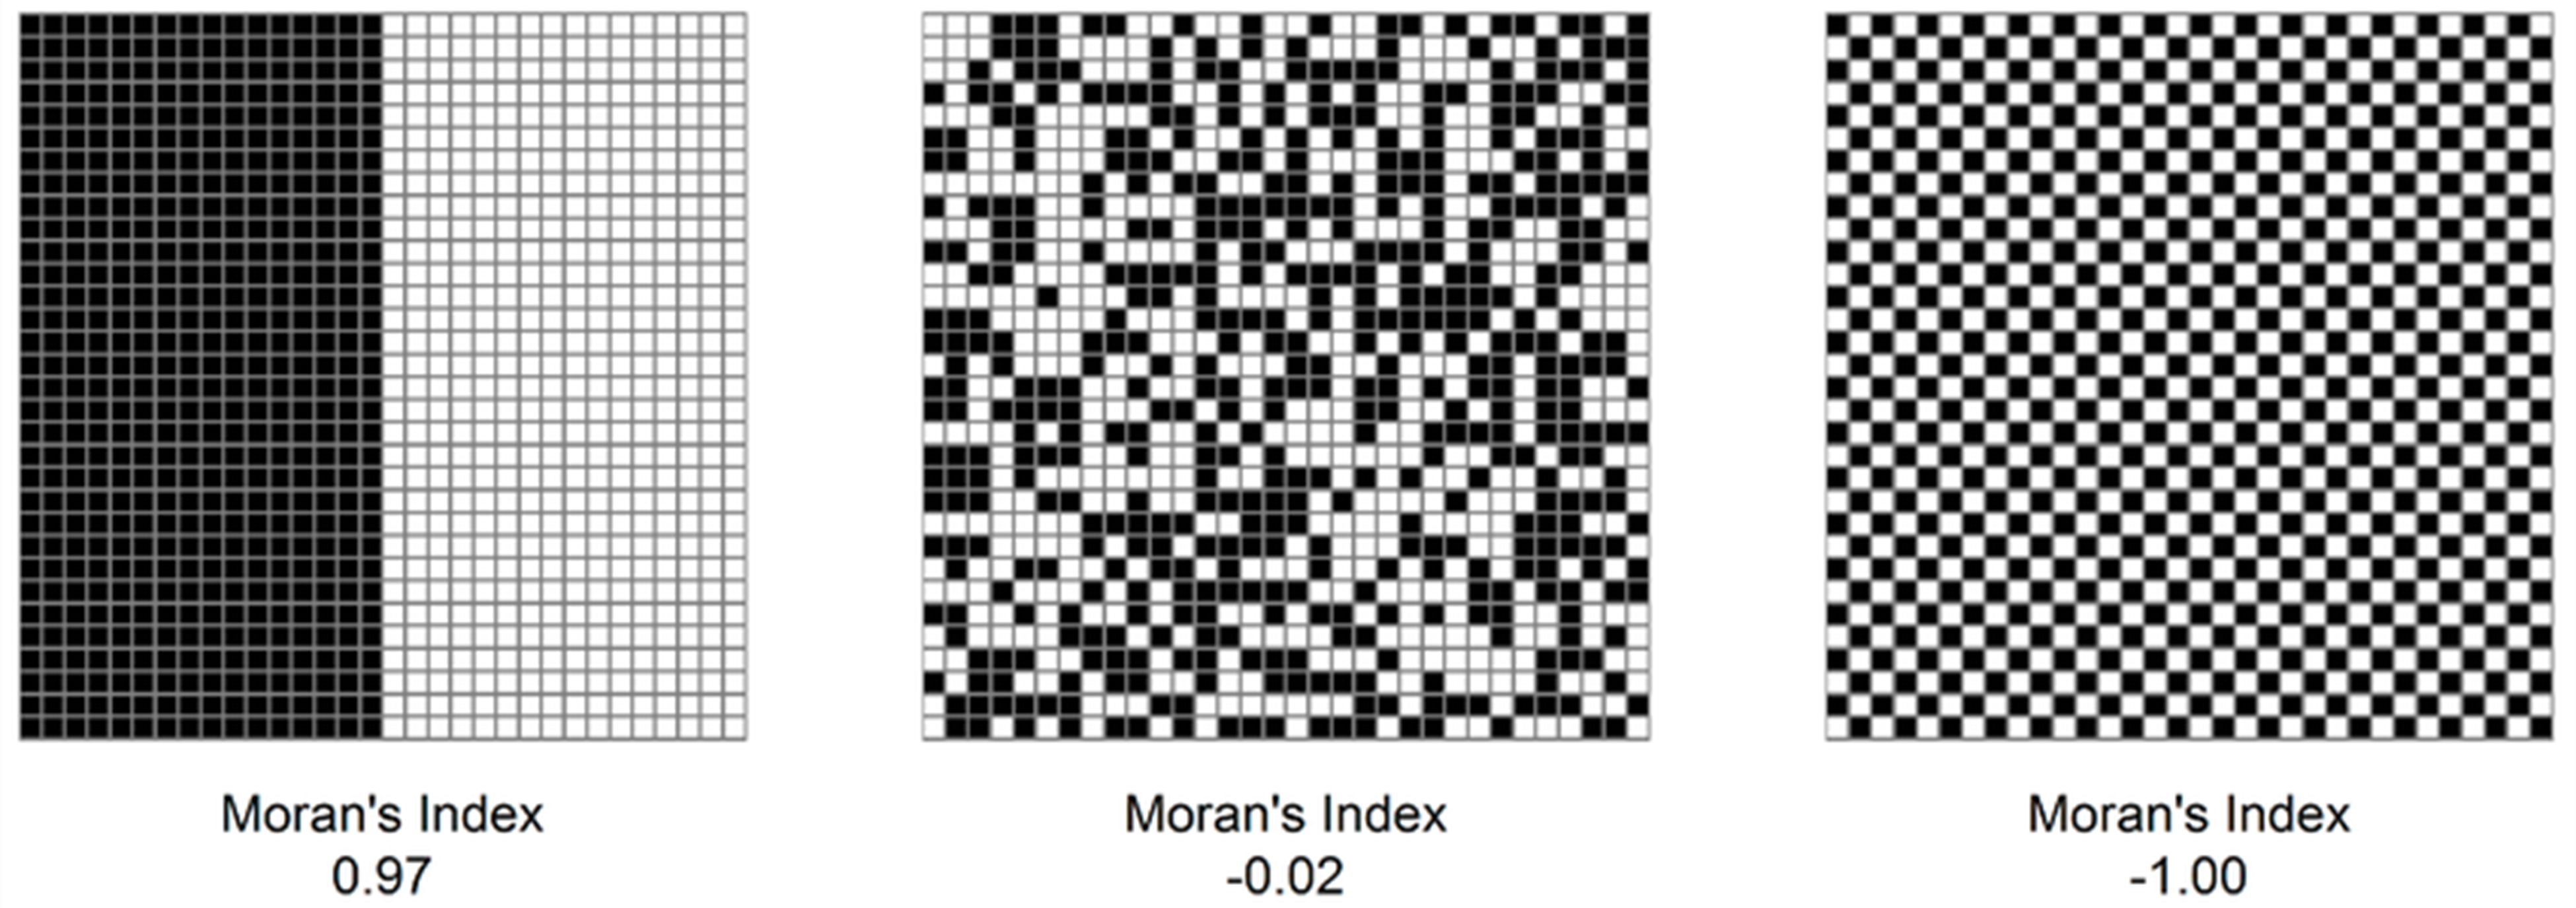
\includegraphics[width=0.75\textwidth]{moran example.png}
    \caption{Moran's I examples. (Böck et al., 2017)}
    \label{fig:moran_ex}
\end{figure}

An inverse Euclidean distance weight matrix was decided with a $16$ pixels radius cutoff as it penalizes distant pixels so key structural differences 
between the two noise types can be accurately captured. The formula is:
\begin{align*}
    w_{i,j}=
    \begin{cases}
        \frac{1}{d_{i,j}}, \quad\text{if } d_{i,j}\le16\\
        0, \qquad\text{otherwise}
    \end{cases}
    \qquad\text{where } d_{i,j} \text{ is the distance between pixel indexed } i \text{ and } j
\end{align*}
It is worth noting that here, the index $i$ and $j$ relates to pixel coordinates with the formula $i=u+256v$. Inversely, $u=i\mod 256$ and 
$v=\lfloor\frac{i}{256}\rfloor$. The complete spatial weight matrix, and thus the Moran's I coefficient will be computed using technology 
(see Appendix REF). 

The final quantitative metric I will use is called the power spectral density, a potent tool in signal processing which quantifies the power 
distribution of a signal across frequencies (Slavič et al., 2021, p.64). For our use case, where the signal is discrete and two dimensional, 
the power spectral density can be expressed as (Blackman \& Tukey, 1958, p.193):
\[P(u,v)=\frac{1}{MN}{\|\EuScript{F}(u,v)\|}^2\]
where $\EuScript{F}(u,v)$ is the 2D Discrete Fourier Transform (DFT) (Gonzalez \& Woods, 2007, p.257):
\[\EuScript{F}(u,v)=\sum_{u=0}^{M-1}\sum_{v=0}^{N-1}f(x,y)e^{-j2\pi\left(\frac{ux}{M}+\frac{vy}{N}\right)}\]
Adapting to this IA, we will firstly substitute $M=N$ due to our square terrain map and secondly, substitute $f(x,y)$ with $\EuScript{N}_{FV}(x,y)$
or $\EuScript{N}_{FP}(x,y)$.

After calculating for all values of $u$ and $v$, plot $\log P(u,v)$ onto the pixel $(u,v)$. Due to the computation-heavy nature of this algorithm, 
the PSD will be done using technology (see Appendix REF).